% !TEX root =  ../main.tex
\section{Results}
\label{sec:results}
In this Section we present some of the results obtained with our planner. The complete sequences computed are shown in the companion video.
Specifically, we demonstrate the planner for two really different robots, in a large variety of environments: the humanoid HRP-2 and the quadruped HyQ.
For each scenario we indicate the chosen heuristics. We also provide a performance analysis, which shows that the planner is compatible with \gls{interactive} applications,
and present the success rates obtained in each scenario. Moreover, we demonstrate the interest of our robustness criterion in the different computed poses.
Finally, a last example suggests possible applications to dexterous manipulation.

In our previous work~\citep{tonneauisrr15} additional results are demonstrated with various virtual avatars (Figure~\ref{fig:robots_old}).
In this extension we choose to focus on actual robots. We invite the interested reader to watch the ISRR video\endnote{https://www.youtube.com/watch?v=LmLAHgGQJGA}, and 
to refer to the previous paper for a discussion on these results.

%~ We say that the planning is \gls{interactive} when the computation time for one step is lesser than the
%~ time to execute it. We arbitrarily approximate this time to one second.

\begin{figure}[t]
\centering
  \begin{overpic}[width=1\linewidth]{figures/robots_old}
		%~ \put (5,) {1)} 
		%~ \put (37,) {2)} 
		%~ \put (68,) {3.a)} 
		%~ \put (5,27) {3.b)} 
		%~ \put (37,27) {4.a)} 
		%~ \put (68,27) {4.b)} 
	\end{overpic}
\caption{Virtual avatars in various scenarios demonstrated in our conference paper.}
		   \label{fig:robots_old}
\end{figure}

\subsection{Description of the scenarios}
In all the scenarios considered, the formulation of the problem is always the same:
a start and goal root configurations are provided as an input of the scenario.
The framework computes the initial contact configuration, and outputs a sequence of contact configurations connecting it to the goal.
In each scenario we detail the parameters chosen: the heuristics, and the constraints on the reachable workspaces (for instance in all the scenarios,
the reachable workspaces of the legs of HRP-2 are always required to intersect with the environment). 
%~ The companion video presents the complete contact sequence obtained in all these scenarios.

% \subsubsection*{Truck egress (Figure~\ref{res_truck_pres} and Figure~\ref{res_truck_bd}) -- Humanoid and insectoid robots.}
%\subsubsection*{Truck egress -- Humanoid and insectoid robots (Figure~\ref{res_truck_bd}).}
\subsubsection{HRP-2 -- Steep staircase (Figure~\ref{fig:stair_robust}):}

\begin{figure*}
  \centering
  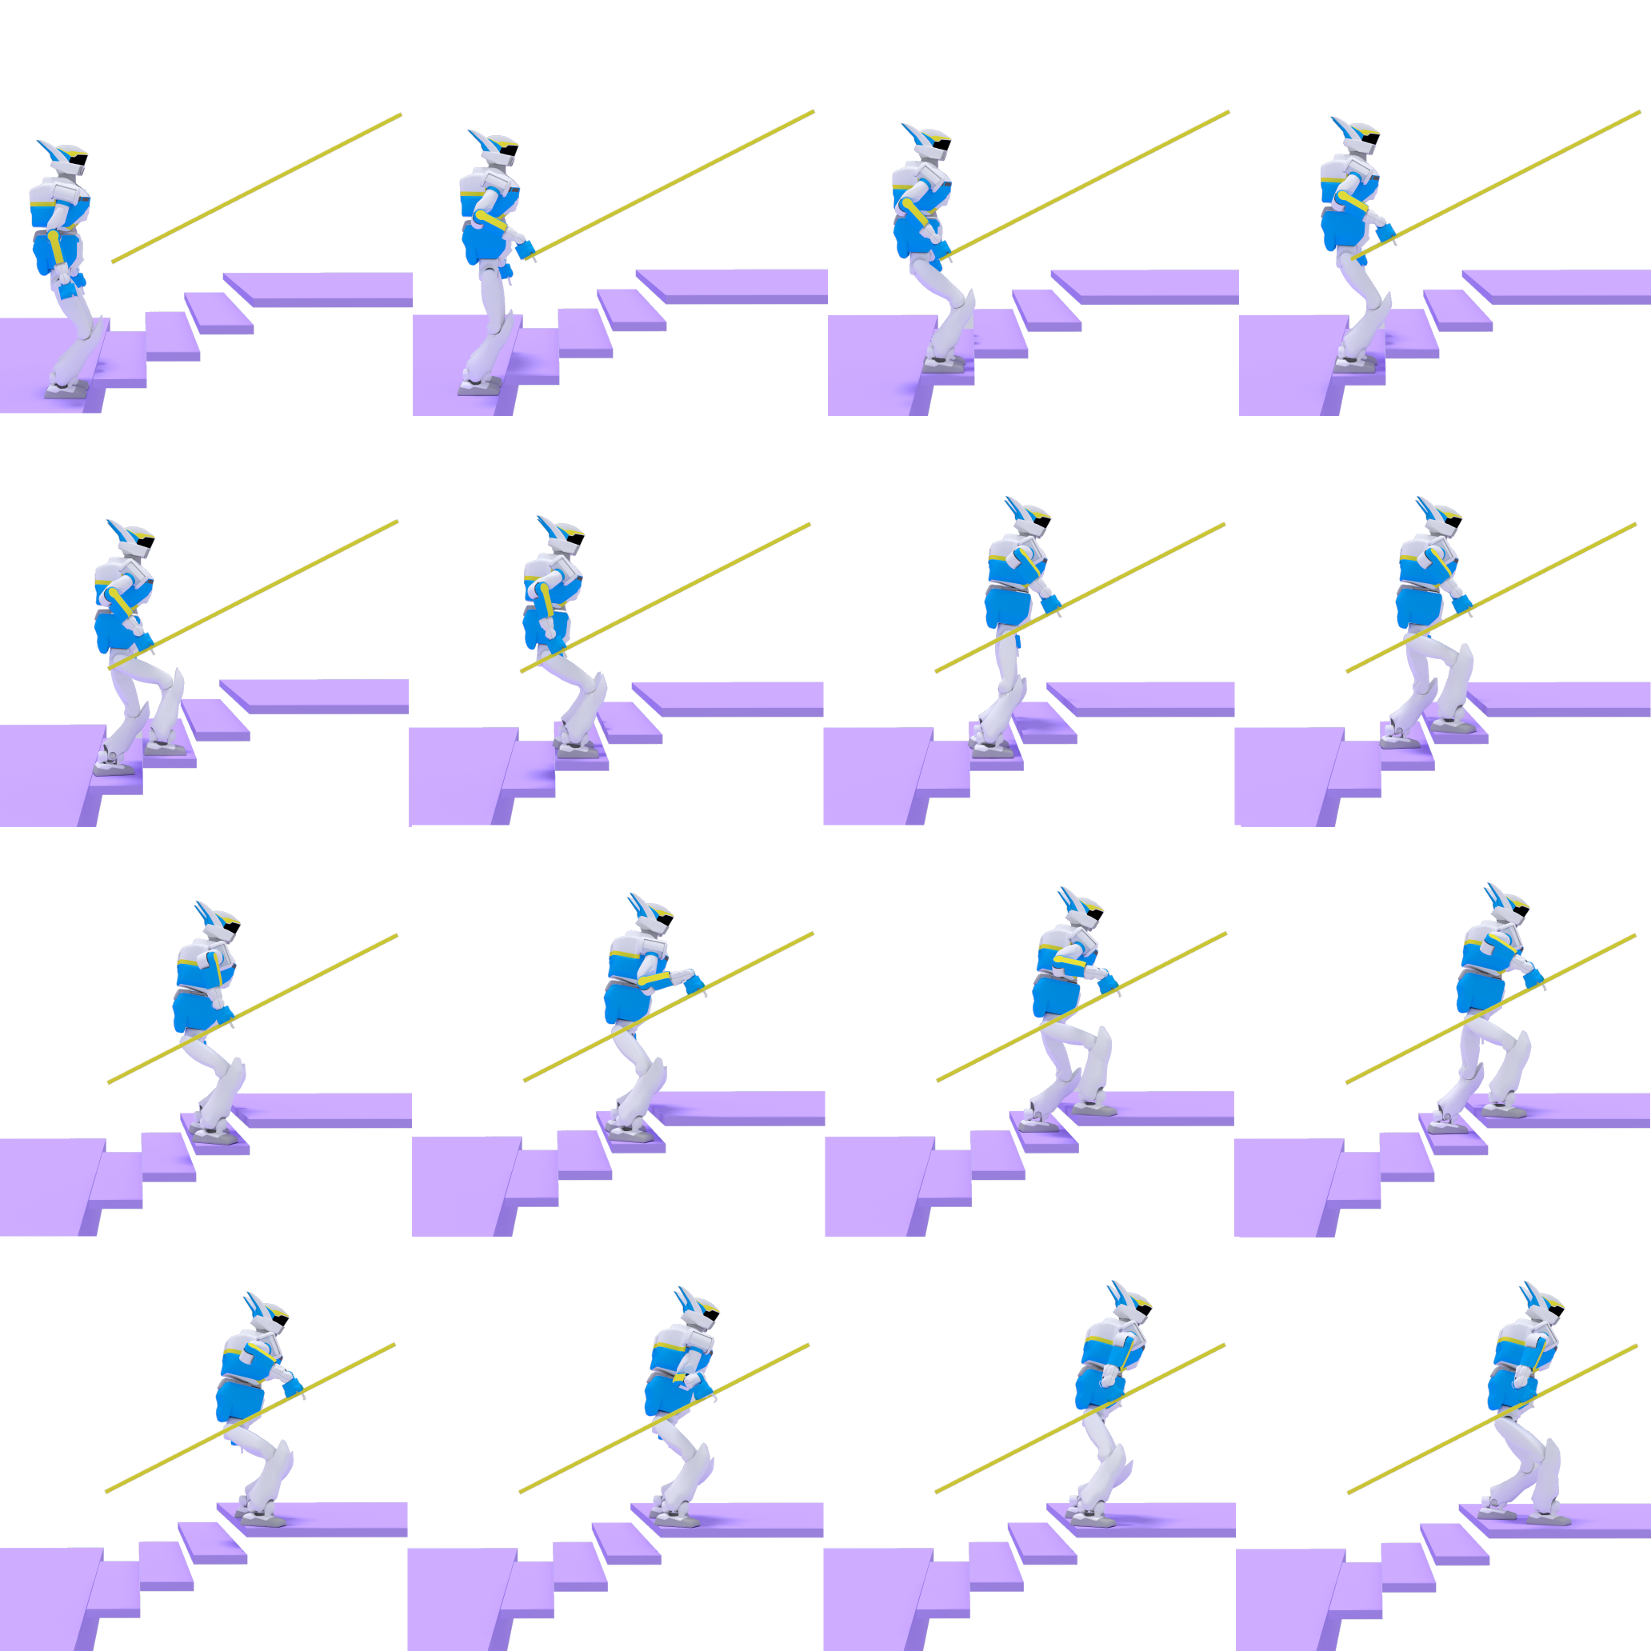
\includegraphics[width=0.5\linewidth]{figures/stair}
  \caption{
           HRP-2 in the steep stair climbing scenario. }
		   \label{fig:stair_robust}
\end{figure*}

The goal is to climb three 15-cm high steps. This height requires HRP-2 to use a ramp to perform the task.

\noindent\textbf{Contacts involved:} Feet and right arm.

\noindent\textbf{Heuristics:} The manipulability $h_w$ is chosen for the feet; $h_{EFORT}$ is chosen for the right arm.
Regarding equilibrium, the video demonstrates two sequences computed for two different threshold values of $b_0$: $0$ and $2$ (Figure~\ref{fig:stair_robust}). 

\noindent\textbf{Observations:}
This scenario illustrates best the importance of the equilibrium-robustness criterion.
With a robust approach, more states are required to reach the last step (15 rather than 13 in average).
However, when the last step is reached by both feet, in the nonrobust case the contacts are extremely close to 
the cone limits (Figure~\ref{fig:stair_comp}).


The geometry of the environment is easily addressed by our planner, and the contact planning is several times faster than real time in this scenario.

Again, the interpolation motion between the contact steps is out of the scope of this paper. However it should be noted that the computed plan in this scenario has been executed successfully on the robot~\citep{Carpentier2016}.

\begin{figure}
  \centering
  %~ 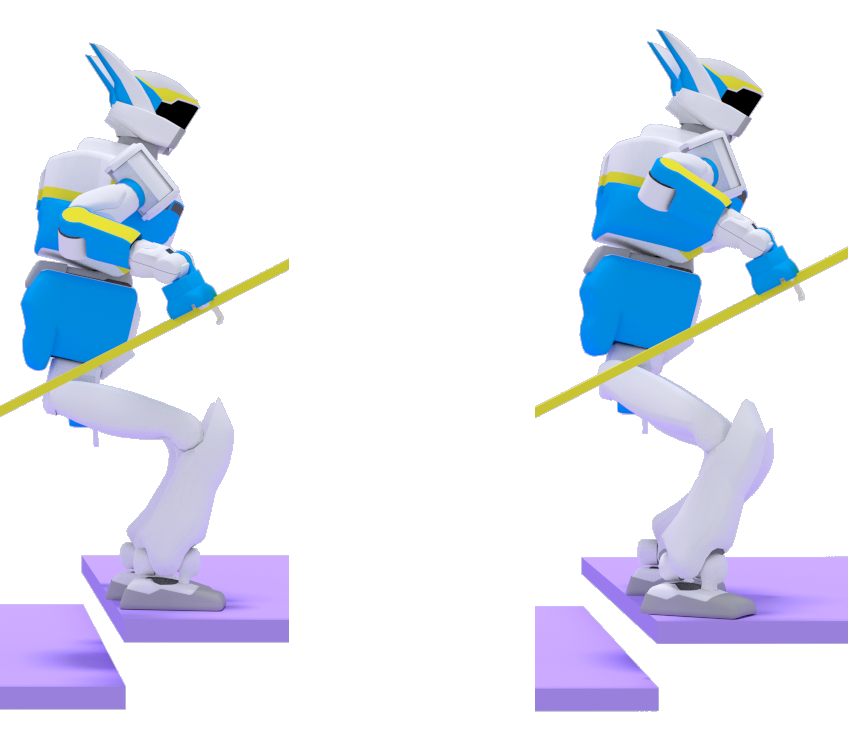
\includegraphics[width=0.6\linewidth]{figures/stair_robust}
  \begin{overpic}[width=0.5\linewidth]{figures/stair_robust}
		\put (17,5) {\small{\color{red}$b_0 = 0.23$}} 
		\put (79,5) {\small{\color{green}$b_0 = 6.16$}} 
		%~ \put (68,) {3.a)} 
		%~ \put (5,27) {3.b)} 
		%~ \put (37,27) {4.a)} 
		%~ \put (68,27) {4.b)} 
	\end{overpic}
  \caption{
           Evaluation of the robustness $b_0$ of two contact configurations. Although in equilibrium, the left configuration is on the verge of slipping.}
		   \label{fig:stair_comp}
\end{figure}

\subsubsection{HRP-2 -- Standing up (Figure~\ref{fig:standing}):}
From a bent configuration, a standing-up motion is computed in a constraining environment.
The resulting motion involves using a wall as support, and climbing a 25-cm high step.

\begin{figure*}
  \centering
  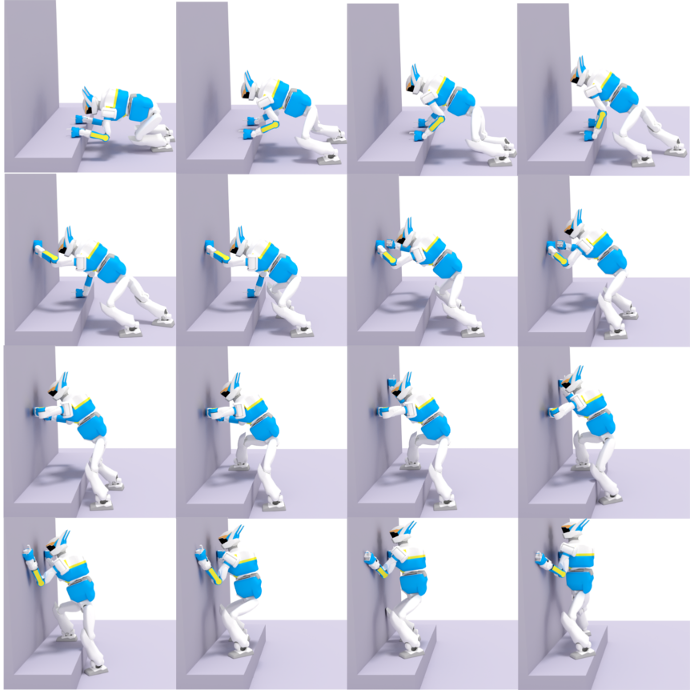
\includegraphics[width=0.5\linewidth]{figures/standing}
  \caption{
           HRP-2 in the standing scenario. }
		   \label{fig:standing}
\end{figure*}


\noindent\textbf{Contacts involved:} All (both feet and hands).

\noindent\textbf{Heuristics:} $h_w$ for the feet, $h_{EFORT}$  for the hands.

\noindent\textbf{Observations:} The scenario illustrates well the acyclic aspect of the planning. For instance, in the four first frames of Figure~\ref{fig:standing}, we can see that the right foot
is moved twice, with the left foot in between, before the configuration allows HRP-2 to move its hand.
Because the contacts are tried in a FIFO manner, the fact that the output contact sequence is acyclic shows that a cyclic approach (with a finite state machine for instance) is not sufficient
for the computed path. The reason for this is not reachability, but equilibrium. The planning is slower than for the stair scenario (because the contact generation fails more),
though it remains compatible with \gls{interactive} performances. % \adnote{Maybe define what you mean by 'interactive' and 'real-time' at some point.}


\subsubsection{HRP-2 -- Car egress (Figure~\ref{fig:car}):}
This scenario is inspired from the Darpa challenge car egress scenario (\url{http://cpc.cx/edH}). HRP-2 has 
to find the contact sequence that allows it to step out of a car.

\begin{figure}
  \centering
  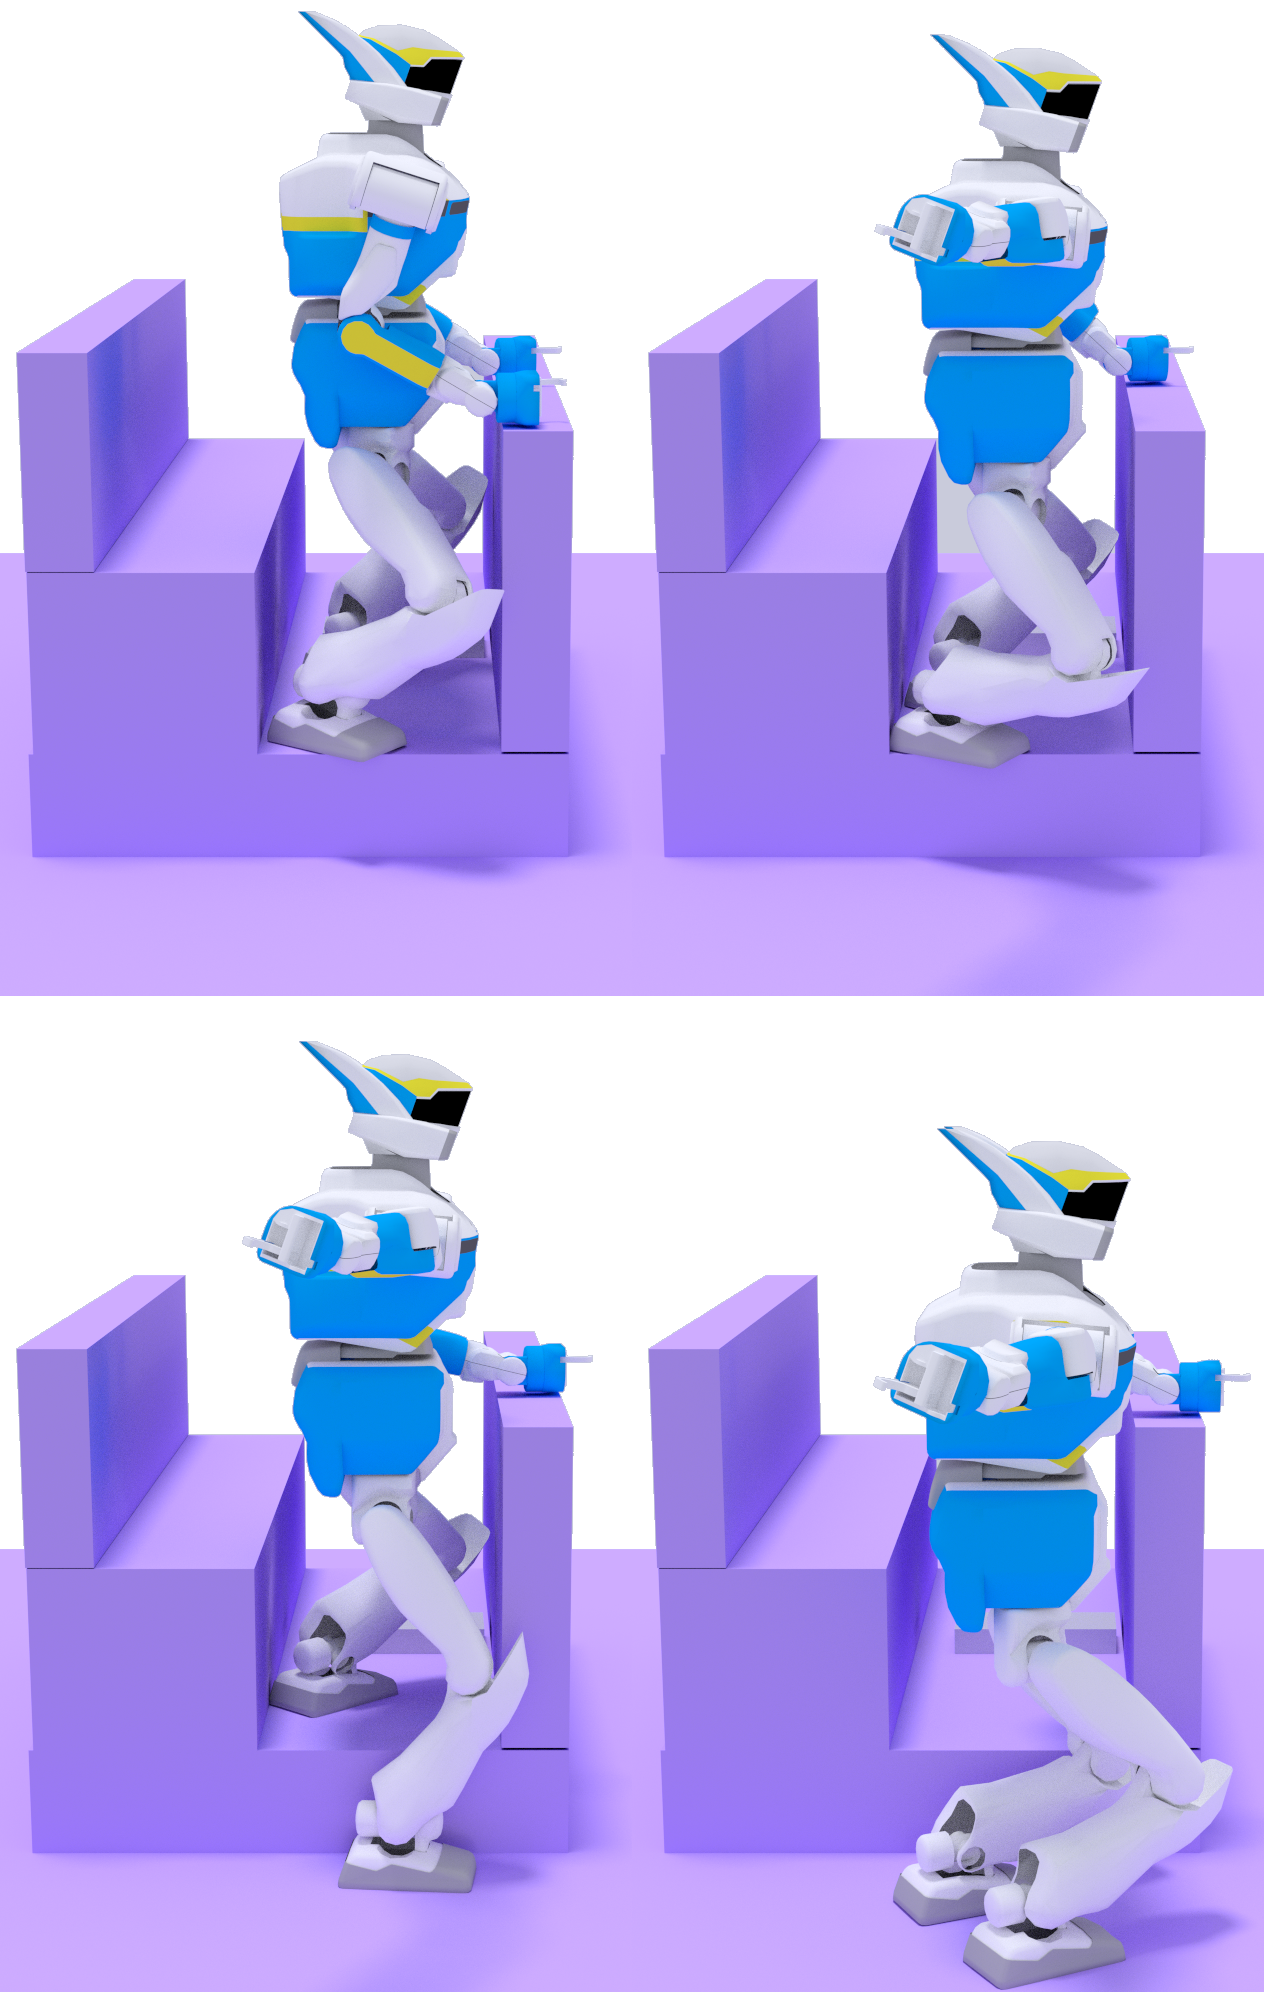
\includegraphics[width=0.5\linewidth]{figures/car}
  \caption{
           Selected frames from the car egress scenario. }
		   \label{fig:car}
\end{figure}


\noindent\textbf{Contacts involved:} All (both feet and hands).

\noindent\textbf{Heuristics:} $h_w$.

\noindent\textbf{Observations:} The difficulty of this scenario lies in the strong reduction of the reachable workspace induced 
by the extreme proximity of all obstacles. The planner is able to find a sequence, that consists in many steps.
The proximity of the obstacles invalidate a large number of contact candidates because of collisions. To avoid breaking more than one contact between each step, the motion has to be decomposed into a large number of steps (61 in average).
While this scenario is the slowest to solve, the planner still computes a solution \glslink{interactive}{interactively}.
 % \adnote{Maybe define what you mean by 'interactive' and 'real-time' at some point.}


\subsubsection{HyQ -- Darpa-style rubble (Figure~\ref{fig:darpa})}
The quadruped robot is given the task to cross a rubble composed of bricks rotated at different angles and directions.

\begin{figure*}
  \centering
  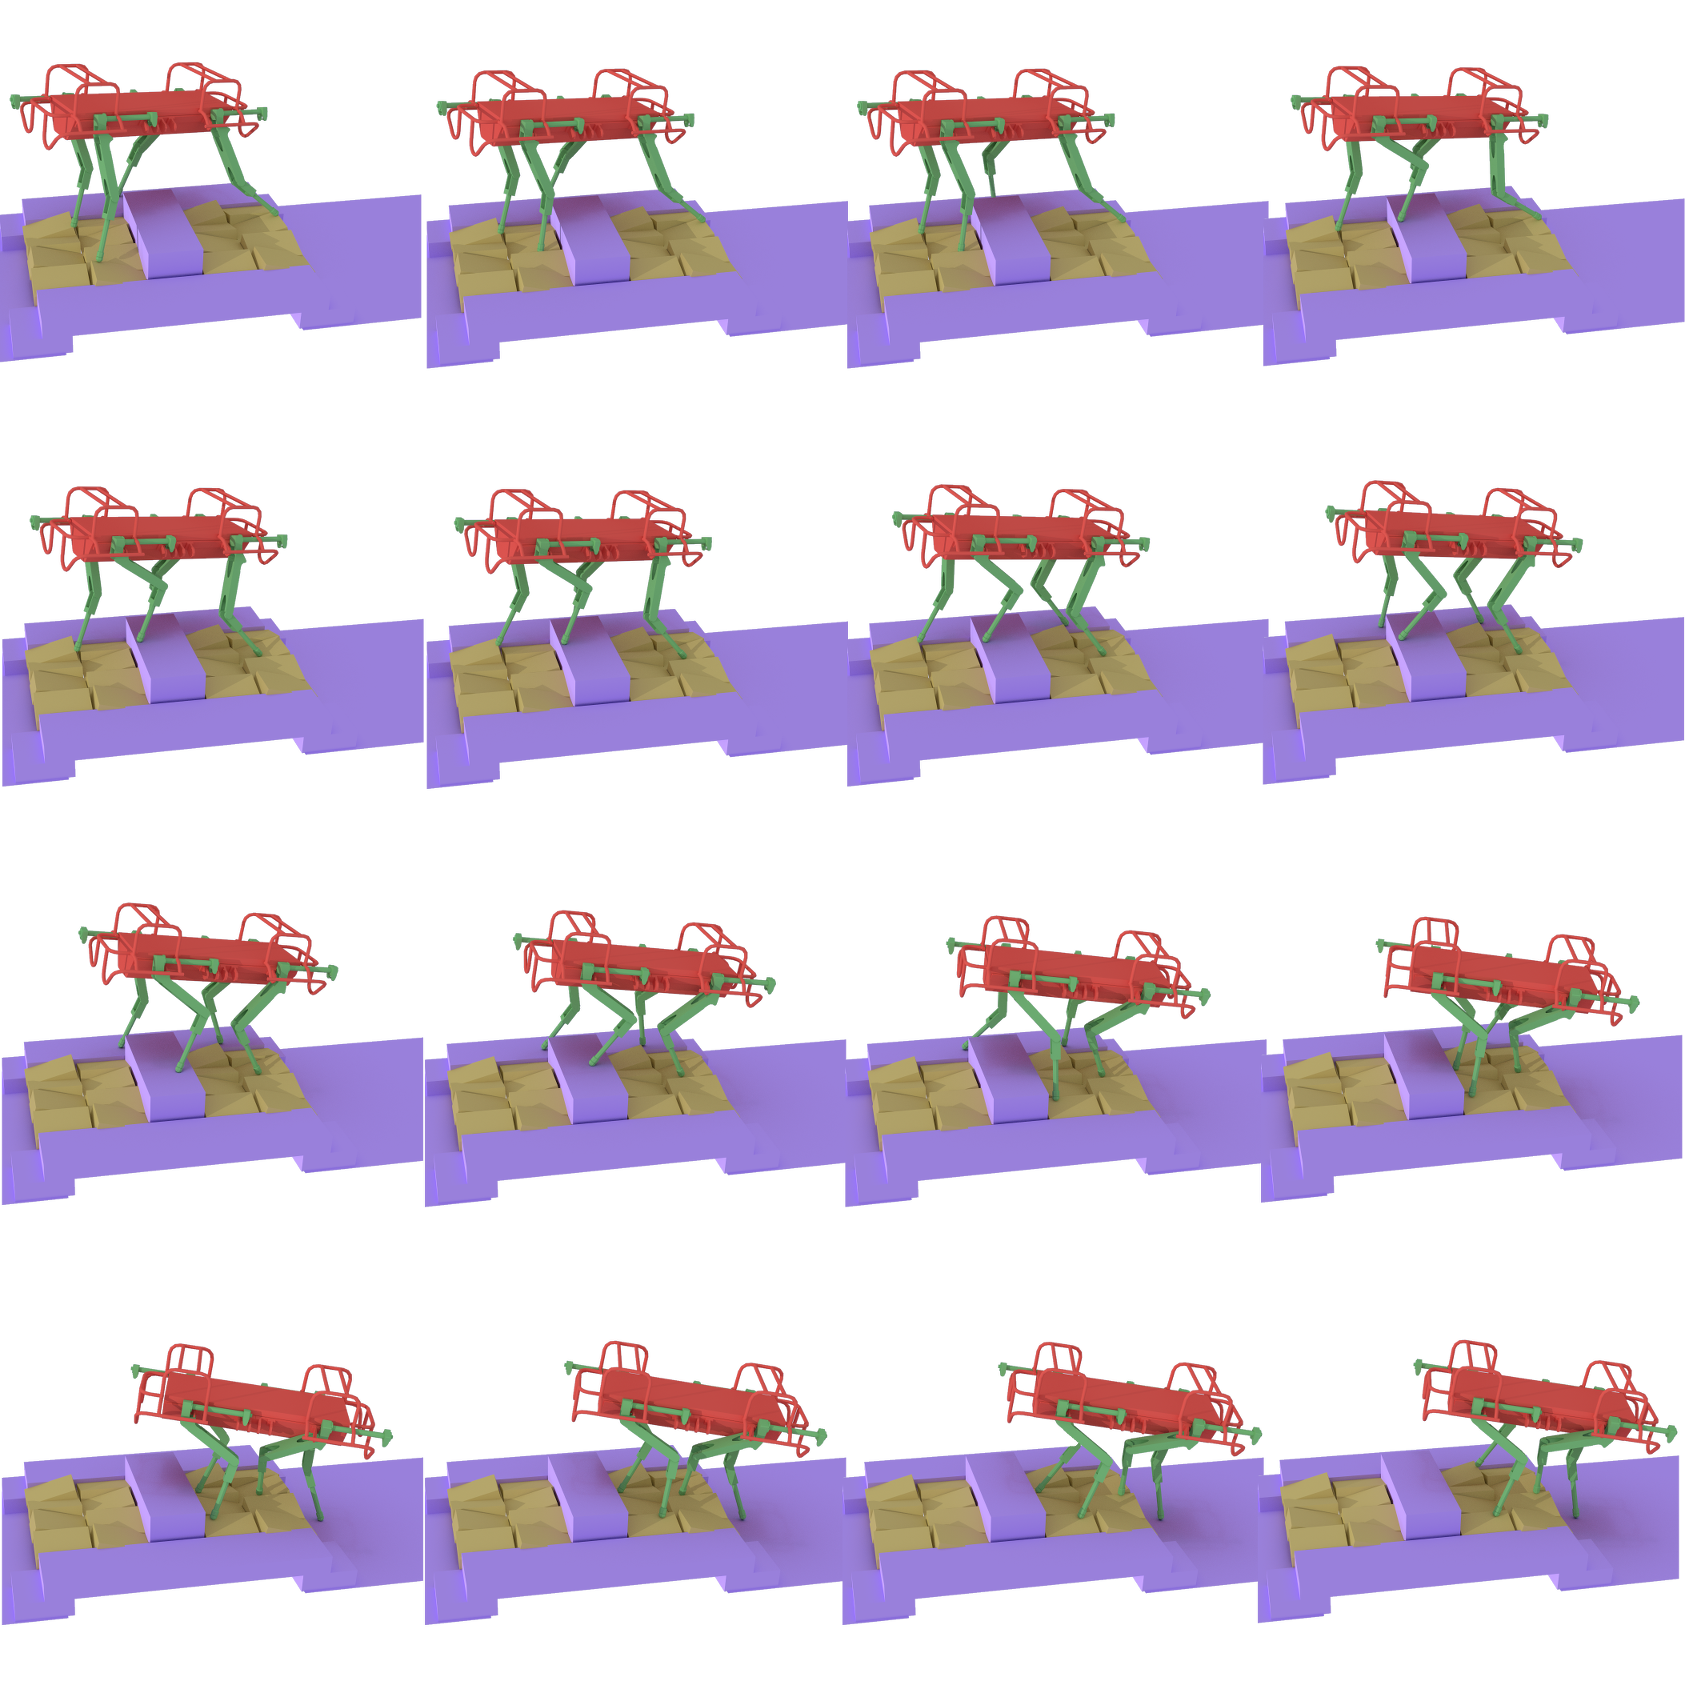
\includegraphics[width=0.5\linewidth]{figures/darpa}
  \caption{
           Robust crossing of rubbles by HyQ ($b_0 > 20$). }
		   \label{fig:darpa}
\end{figure*}


\noindent\textbf{Contacts involved:} All (the 4 legs).

\noindent\textbf{Heuristics:} $h_w$ for all legs. The robustness threshold $b_0$ is set to $20$.

\noindent\textbf{Observations:} In this context, setting up a really important minimum value for $b_0$ is possible due to the high
stability of the HyQ robot, and results in more contact switches, in exchange for safety. The path-planning takes a few seconds due to the constraint that the 4 reachable workspaces of all legs must
collide with the environment at all times. %\adnote{Why do not relax this constraint and require only 3 legs?} 
Again, the computation times remain however \gls{interactive}.

\subsubsection{HyQ -- Obstacle race (Figure~\ref{fig:HyQ_bridge} and~\ref{fig:HyQ_obs}):}
In this long scene, HyQ is first required to cross a 55-cm large hole; then, to cross a narrow ``bridge'', only 25-cm large.

\begin{figure}
  \centering
  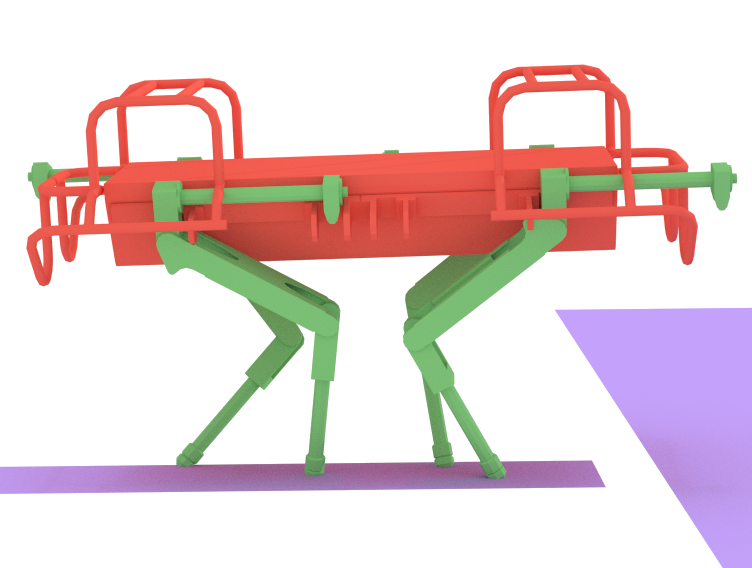
\includegraphics[width=0.4\linewidth]{figures/HyQ_bridge}
  \caption{
           HyQ crossing a narrow bridge. }
		   \label{fig:HyQ_bridge}
\end{figure}

\begin{figure*}
  \centering
  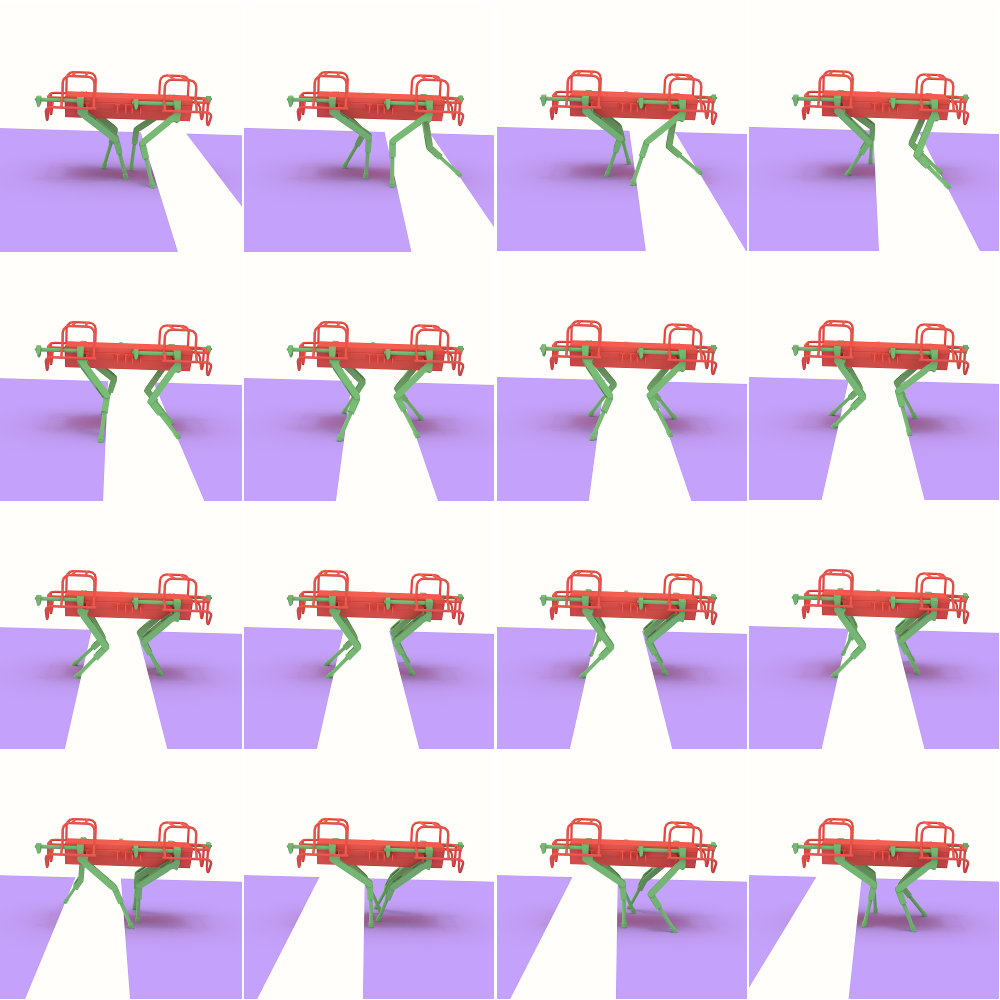
\includegraphics[width=0.5\linewidth]{figures/HyQ_obs}
  \caption{
           Crossing a hole contact sequence for HyQ ($b_0 > 4$). }
		   \label{fig:HyQ_obs}
\end{figure*}



\noindent\textbf{Contacts involved:} All (the 4 legs).

\noindent\textbf{Heuristics:} $h_w$ for all legs. The robustness threshold $b_0$ is set to $10$.

\noindent\textbf{Observations:} Despite the apparent simplicity of the scene, this scenario is a hard case for a contact planner.
While finding a guide path above the hole is easy for the guide planner, finding a sequence of contacts that allows for equilibrium is not trivial.
Second, the narrow bridge is hard both for the planner and the contact generator: to make sure that equilibrium is preserved along the traversal,
the bridge must be approached with the appropriate angle.
The difficulty is illustrated in Figure~\ref{fig:HyQ_obs}, where several feet rearrangements are required to cross the hole (although the video shows this best).
The planner however succeeds in finding a feasible sequence in the end, again with \gls{interactive} computation times.

\subsubsection{HRP-2 -- Path re-planning (Figure~\ref{fig:re-planning}):}
In this long scene, HRP-2 plans a path through several obstacles. the scene is edited during the execution of the motion: a stair is added,
some stepping stones are removed, and part of the final staircase is deleted. All these modifications require re-planning.


\begin{figure}
  \centering
  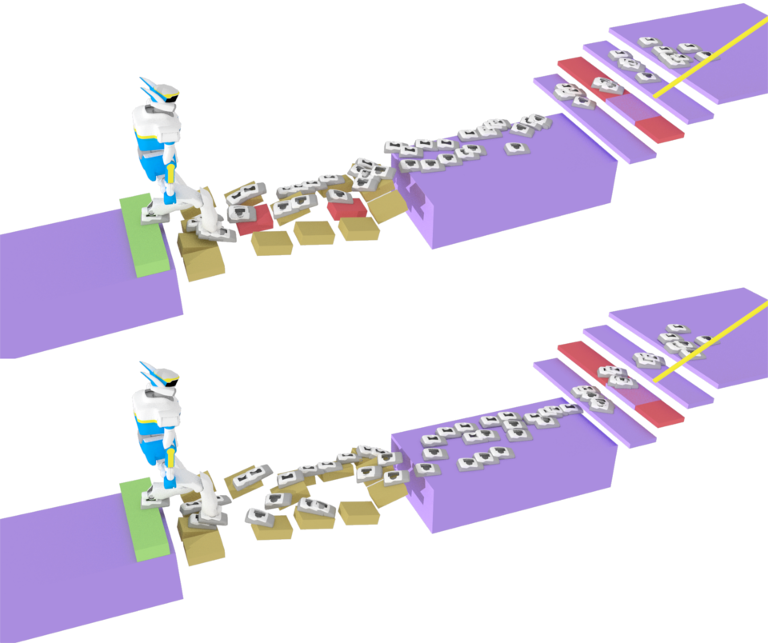
\includegraphics[width=0.7\linewidth]{figures/replanning}
  \caption{
           HRP-2 in the re-planning scenario. After the red step stones are removed, a new sequence of contacts is re-planned. Hand contacts
           are not presented here for readability.}
		   \label{fig:re-planning}
\end{figure}

\noindent\textbf{Contacts involved:} Feet and the right arm.

\noindent\textbf{Heuristics:} $h_w$  for all legs. $h_{EFORT}$  for the right arm. The robustness threshold is set to $2$.

\noindent\textbf{Observations:} This scenario is designed to illustrate concretely the computation times of the planner.
In the video, the footsteps indicating the contact sequence appear at the average speed of their computation (including the guide-path planning).


\subsubsection{3-fingered hand -- Manipulation of a pen (Figure~\ref{fig:penrot}):}
This scenario is proposed to illustrate the generality of our approach: we consider a manipulation task for a robotic hand and use
our contact planner to compute a contact sequence for the fingers, considered as effectors (Figure~\ref{fig:penrot}).
Although we do not address the hard issue of accounting for rolling motions, the planner is able to compute the shown sequences in less than 5 seconds.

\begin{figure*}
\centering
  \begin{overpic}[width=1\linewidth]{figures/penrot}
	\end{overpic}
\caption{Contact sequence found for a pen manipulation in a zero gravity environment.}
		   \label{fig:penrot}
\end{figure*}

 
\noindent\textbf{Contacts involved:} Three finger-tips.

\noindent\textbf{Heuristics:} $h_{EFORT}$ for all fingers.
 
 
\subsection{Influence of the parameters} \label{sec:influence}
This subsection discusses the several factors that influence the outcome of our planner: the root scaling factor $s$, the choice of heuristics for
contact generation, the desired value of the robustness parameter $b_0$, and lastly, the discretization 
of the guide path.
 
\subsubsection{Choosing the scaling factor $s$} \label{sec:params}
To find a convenient value $s^*$ of $s$, we proceeded as follows. 
For several values of $s$, we generated $10 000$ configurations. 
We then computed the rates of false positives (i.e. the configuration satisfies
the reachability condition, but does not belong to \gls{ccequil0}) and false negatives (i.e. the configuration does not satisfy the 
reachability condition, but belongs to \gls{ccequil0}).

The obtained results for HRP-2 are summarized in Table~\ref{tab:scale}, averaged over all scenes (except for the car egress: in this scenario, 
statistical tests are not really conclusive since we are only interested in a small area of the environment).
As it can be expected, the scaling results in a high increase of the false negatives, while the false positives decrease.
For HRP-2 we decided to set $s^*=1.2$, that results in less than 3 \% of false positives, and was also effective
for the car egress scenario. 

\begin{table}
\centering
\footnotesize
\begin{tabular}{c | c | c}
   Value of $s$ &  False positive & False negative\\
 \hline
   1   & 24\% & 0 \%\\
   1.1& 12\% & 4\% \\
   1.15& 7\% & 6\%\\
   1.2 & 3\% & 7.5\%\\
   1.25& 2\% & 8.3\%\\
   1.5 & 1\% & 9.5\%\\
 \end{tabular}
\caption{Percentage of true and false positive in the reachability condition, depending on the scaling value of $W^0$.}
\label{tab:scale}
\quad
\end{table}

\subsubsection{On the choice of heuristics} \label{sec:heuristichoices}
In our conference paper, the computed motions were only generated using the EFORT heuristic.
EFORT is designed for tasks requiring to exert important forces (such as pushing / pulling / climbing). 
Regarding locomotion tasks, such as the stair scenario, one issue with EFORT is that it tends to generate
configurations close to singularities (and joint limits). While this does not significantly impact
the generation of the plan, the resulting interpolation on the real robot turned out to be harder \citep{Carpentier2016}.
For this reason, we now prefer to use our manipulability-based heuristic for the legs of the robot, but we still
use EFORT for the arms, that results in less contact repositioning.

\subsubsection{On the robustness equilibrium criterion} \label{sec:parrob}
Robustness is really important when considering practical applications on the robot, to account 
for the various uncertainties that result from environment and state estimation. However,
maximizing the robustness criterion is not necessarily optimal, because the resulting configurations may be too conservative, thus not favoring the motion. In our experiments, we choose not to maximize the robustness,
but to empirically set a robustness threshold value under which a configuration is not considered to be in
static equilibrium (If no candidate reaches the threshold, instead of failing, the algorithm can eventually return the ``more robust'' configuration
found). Currently for HRP-2, a threshold value of 2 subjectively gives the best results in the considered scenarios, while 10 seems to be a good choice for HyQ. Both values do not
significantly slow down the planning times.

\subsubsection{Discretization of the guide path} \label{sec:disc}
Currently, to discretize the path, the user defines a fixed step size. The step size
has an influence on the output of the planner: if too large steps are taken,
the planner may fail since we impose the constraint that only one contact change might occur
between two consecutive steps. For instance, in most scenarios the torso of HRP-2 moves about 15 cm between two postures, but only 3 cm
for the car egress scenario, where we had to lower the step size because of the many contact breaks induced by the extremely constraining geometry.
For future work, we would like to automatically adapt the size of the discretization step to the complexity of the planning, for instance
by reducing the step size when failure occurs.

\subsection{Performance analysis} \label{sec:perf}
To analyze performance, for each considered scenario, we ran the simulation 1000 times.
We measured the computation time spent in each aspect of the algorithm, and also analyzed the success
rate obtained for each scenario.


\begin{table*}
\centering
\footnotesize
\begin{tabular}{ >{\centering\arraybackslash}m{37pt} | >{\centering\arraybackslash}m{57pt} | >{\centering\arraybackslash}m{65pt} | >{\centering\arraybackslash}m{70pt} | >{\centering\arraybackslash}m{73pt} | >{\centering\arraybackslash}m{80pt} | >{\centering\arraybackslash}m{10pt}}
  Scenario (nb steps) &  Complete guide generation (ms) & Static equilibrium (ms) & Collision (ms) & Inverse Kinematics (ms) & Total generation time (ms) & Time per step (ms)\\
 \hline
   Stairs (18) & 6 -- \textbf{13} --  24 & 13 --  \textbf{32} -- 329   & 1 --  \textbf{4} -- 38 & 26 --  \textbf{127} -- 1345 & 92 --  \textbf{261} -- 2174 & \textbf{14} \\
   Standing (24)& 4 -- \textbf{451} --  985 & 27 --  \textbf{144} -- 338   & 2 --  \textbf{12} -- 37 & 144 --  \textbf{1046} -- 2374 & 310 --  \textbf{1622} -- 3429 & \textbf{66}  \\
   Car (61)& 1 -- \textbf{529} --  995 & 64 --  \textbf{85} -- 144   & 394 --  \textbf{735} -- 1422 & 3947 --  \textbf{13069} -- 36262 & 6775 --  \textbf{20890} -- 52963 & \textbf{342} \\
   Rubble (71)& 3 -- \textbf{524} --  993 & 242 --  \textbf{511} -- 3480   & 233 --  \textbf{505} -- 4564 & 180 --  \textbf{414} -- 3518 & 1400 --  \textbf{3058} -- 13126 & \textbf{43} \\
   Race (112)& 1 -- \textbf{501} --  995 & 266 --  \textbf{449} -- 3956   & 824 --  \textbf{1061} -- 2130 & 666 --  \textbf{874} -- 1613 & 2530 --  \textbf{3722} -- 10030 & \textbf{33}
   %Standing up & $70$ & 23 & 48\\
 \end{tabular}
\caption{minimum, \textbf{average} and worst time (in ms) spent in the generation process for each scenario and each critical part of the generation process. The last
column indicates the average time necessary to compute one contact transition.}
\label{tab:requestime}
\quad
\end{table*}


\begin{table*}
\centering
\begin{tabular}{ l | >{\centering\arraybackslash}m{65pt} | >{\centering\arraybackslash}m{65pt} | >{\centering\arraybackslash}m{65pt} | >{\centering\arraybackslash}m{65pt} | c}
  &  Path planning & Equilibrium feasibility & Kinematic failure & Equilibrium failure \\
 \hline
   Steep stairs & 100\%  & 99.5\% & 0.1\% & 0.4\% \\
   Standing up & 68\% & 87.8\% & 6.1\% & 6.1\% \\
   Car egress & 39\% & 77.0\% & 21.0\% &  2.0\% \\
   Rubble & 74\% & 97.9\% & 0.1\% & 2.0\% \\
   Obstacle race & 58.0\% & 95.7\% & 1.8\% & 2.5\% \\
 \end{tabular}
\caption{Success rates for each scenario, rounded to the first decimal. The first value indicates the percentage of successful complete contact plannings for 1000 tests; The second value
indicates the percentage of equilibrium feasible root configurations: considering each limb individually, indicates the percentage of root configurations of the guide path that
led to a feasible contact. Kinematic failure is the percentage of contact generations that failed because no collision-free candidate was found. Equilibrium failure is the percentage of contact
generations that failed because no candidate respected the static equilibrium condition.}
\label{tab:requestpercent}
\quad
\end{table*}

\subsubsection{Computation times}
Table~\ref{tab:requestime} summarizes the performance measurements obtained, in terms of computation times.

Considering the repartition of the computation time, for HRP-2, most of the time is spent performing inverse kinematics.
This is not surprising considering the number of calls to the methods: IK projection is used intensively to maintain contact continuity between two postures; 
it is also applied every time a new candidate needs to be evaluated. In particular for the car egress scenario,
the kinematic constraints are really strong. Therefore a large number of projections fail because of joint-limit violations.

For HyQ, there is a more uniform repartition of the times for the rubble scenario. For the obstacle scenario,
we observe a large increase of the time spent performing collision checking and inverse kinematics. This is explained
by the complexity of crossing the bridge: the robot has to stand high and create contacts close to each other because
the bridge is narrow. In many cases this results in collisions, thus a large number of contacts have to be evaluated.

In all scenarios, one can observe that the average computation time for one single step is largely below one second,
thus allowing to consider \gls{interactive} applications. 


\subsubsection{Success rates}
Table~\ref{tab:requestpercent} summarizes the success rates obtained for each scenario.
We observe that, as expected, our planner does not succeed systematically, because of the approximations made in our formulation. The extreme situation of the car egress scenario provides the less satisfying results in terms of kinematic failure. This is not
surprising considering the narrowness of the scene.
From a pragmatic point of view, regarding the computation times, we claim that our approach provides a satisfying compromise between completeness and efficiency.
Indeed, the advantage of the framework is that when the contact generation fails, it does so rapidly, which allows us to rapidly re-plan a new contact sequence with a reasonable chance of success.
The most efficient (and immediate) approach is probably to launch in parallel several instances of the planner for a given problem (our current implementation is single threaded) and to apply any successful result.

\begin{table*}
\centering
\begin{tabular}{ c | c | c | c | c }
 Scenario & Method  & Guide Path & Contact sequence & Interpolation \\
 \hline
   \multirow{3}{*}{Stair 20 cm} & \citeauthor{Hauser06usingmotion} &  \multicolumn{3}{c}{5.42 min}  \\
							 & \citeauthor{Mordatch:2012:DCB:2185520.2185539} &  \multicolumn{3}{c}{2 to 10 min} \\
							 & \textbf{Ours} + \citeauthor{Carpentier2016}  & $\mathbf{<}$ \textbf{2 ms} & $\mathbf{<}$ \textbf{14 ms} & $ <$ 2s \\
 \hline
   \multirow{3}{*}{Stair 30 cm} & \citeauthor{Hauser06usingmotion} &  \multicolumn{3}{c}{4.08 min}  \\
							 & \citeauthor{Mordatch:2012:DCB:2185520.2185539} &  \multicolumn{3}{c}{2 to 10 min} \\
							 & \textbf{Ours}  & $\mathbf{<}$ \textbf{2 ms} & $\mathbf{<}$ \textbf{14 ms} & X \\
 \hline
   \multirow{3}{*}{Stair 40 cm} & \citeauthor{Hauser06usingmotion} &  \multicolumn{3}{c}{10.08 min}  \\
							 & \citeauthor{Mordatch:2012:DCB:2185520.2185539} &  \multicolumn{3}{c}{2 to 10 min} \\
							 & \textbf{Ours}  & \textbf{5 s} & \textbf{3 s} & X \\
 \hline
   \multirow{2}{*}{Table (car) egress} & \citeauthor{Bouyarmane2009, DBLP:conf/iser/EscandeKMG08} & 10 min & \multicolumn{2}{c}{3.5 hours}  \\
							 & \textbf{Ours}  & \textbf{529 ms} & \textbf{$<$ 21 s} & X \\
 \end{tabular}
\caption{TODO VERIFIE STATS A LA MAISON.}
\label{tab:compprev}
\quad
\end{table*}
\subsection{Comparison with previous work} \label{sec:compa}
Comparing our method with others is not trivial. Indeed, we focus on the contact planning aspect of the problem, and do not address
the interpolation in this paper, nor provide a strong guarantee that our sequences can be interpolated.
Most papers in the literature only provide the overall computation
time, without specifying how much is spent in each phase. Due to the complexity
of the existing approaches,  we cannot afford the development resources required to reimplement them.

Furthermore, the interpolation itself is not completely solved. For instance in \cite{DBLP:conf/iser/EscandeKMG08}, the end-effector trajectories are computed automatically with splines, but are manually corrected if they enter in collision. In \citep{Mordatch:2012:DCB:2185520.2185539}, internal joint collisions can occur in the resulting motion.
Recent methods suffer from similar issues \citep{Carpentier2016}.


Nonetheless, we indicate in Table~\ref{tab:compprev} what is actually computed by each method and in how much time.
We compare motions obtained in previous works with HRP-2 (or a humanoid avatar) with ours.
The two scenarios we selected consist in:  climbing one step, of height 20, 30 or 40 centimeters; 
getting out of a table, that we consider of a complexity similar to the car egress scenario (or inferior since the feet locations remain on the ground in the former case).
For scenarios that apply, we also indicate the interpolation time that we obtained by feeding the plan to our interpolation method presented in \cite{Carpentier2016}.

Despite the difficulty of comparing the methods, we believe the results presented in Table~\ref{tab:compprev} indicate that our planner holds the promise of planning complete trajectories significantly faster than previous works.



